\chapter{Discussion of Alternatives}
For each step in the \ac{CRISP-DM} process, a multitude of different approaches can be employed. In this chapter, the alternatives are presented and evaluated on the basis of established criteria.

\section{Dataset selection}

	The dataset is the fundament of a data-science project. The quality, size and closeness to reality decide the degree to which the findings can be helpful for solving real problems. 
	In this section, a classification for data-science projects is introduced.
	
	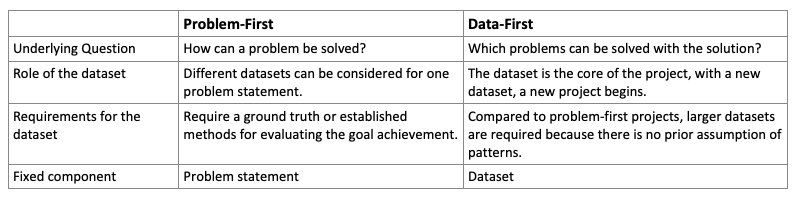
\includegraphics[height=4cm]{Bilder/meta_project.png}
	
	The problem-first project type is characterized by a predefined problem statement or research goal. The underlying question is, how a specific or a set of problems can be solved. For the selection of the dataset, this requires that goal achievement can be measured with existing ground truth. In some cases, also other methods such as expert judgements can be sufficient. In a problem-first project, different datasets can and should be considered.
	
	The complementary project type is the data-first project, which describes most data-mining projects. This type is characterized by a more explorative approach, and the goal to find problems and patterns. Here, the dataset is at the core of the project and the fixed aspect of a project. In turn, this means swapping the dataset is the start of a new project.
	
	With the project type as a decisive factor for the dataset explained, the other evaluation criteria for the dataset is described. In the corporate environment two fundamental sources for data exist. 
	
	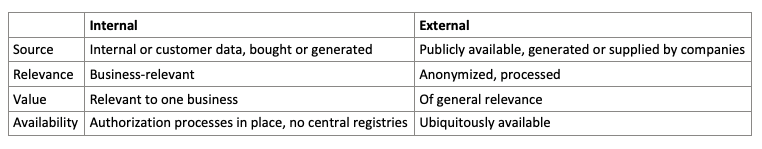
\includegraphics[height=3cm]{Bilder/internal_external.png}
	
	Firstly, data can be sourced from inside the company. This can include customer data or data generated from observation and monitoring processes inside the company. Data is either directly or very closely related to the company's business. Depending on the solution, it can be of use to customers or it can be utilized inside the company. Internally sourced data is almost exclusively rated confidential, limiting even intra-company access to it. Authorization processes and more than often not existing registries for data may hinder project progress.
	
	Secondly, data can be sourced outside the company. A vast number of online registries for data exist, both with paid and free of charge service offerings. Data sources include real-life data and data generated for educational purposes. Because of its publication, the data is stripped from all parts which could expose confidential information such as corporate secrets. Additionally, data is anonymized and processed to limit the usefulness to potential competitors.
	
	It can be stated, that both sources are suited for different goals. 
		
\section{Data Retrieval}
	- how is the dataset stored?

\section{Business Understanding}

	- why did i decide for clustering?

\section{Data Understanding}
	- different data exploration tools can be used for the data understanding.

\section{Data preparation}
- transforming json documents into dataframe rows

- removing stopwords from several languages

- removing numbers and interpunction

- tokenization

	\subsection{Data processing and data wrangling}
	
	
	\subsection{Data cleaning}
	
	\subsection{Feature Extraction and Feature Engineering}
	The majority of pupular ML algorithms require the input of scalar, vector or matrix data. A form of ML models, which work with textual input will be discussed later in this section. 
	But since many algorithms were not designed to work with textual data, a transformation is required before already existing algorithms can be applied. Several methods for representing text as mathematical object will be discussed in the following.

		\subsubsection{One-hot encoding}
		

		\subsubsection{Bag of Words Model}
		Following three documents will be considered to explain the workings of the \ac{BoW} model:

		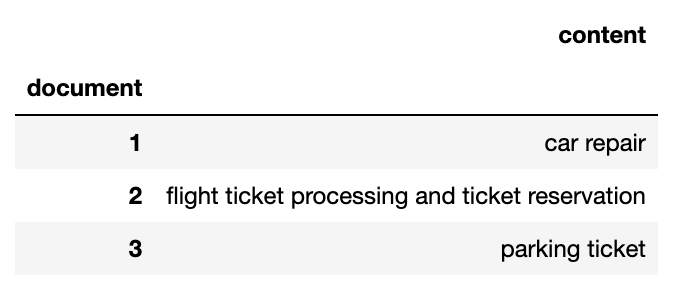
\includegraphics[height=3cm]{Bilder/corpus_bow.png}
		
		A corpus is transformed into the \ac{BoW} representation in two steps. 
		
		Firstly, the vocabulary is determined. 
		The vocabulary is a collection of all words occuring in the corpus. Every word is contained exactly once, regardless of the actual number of occurrences. The vector represenation of one document is of the same length as the vocabulary. One document being represented by one vector, a corpus of several documents can be represented as a matrix. The resulting matrix has the size $ |D|*|V| $, with $|D|$ being the number of documents in the corpus, and $|V|$ being the size of the vocabulary.
		
		Secondly, for each combination of one document $ d_{i} $ and one word $ v_{j} $ in the vocabulary, the occurrences are counted. The times, how often the specific word is contained in the document is noted in the matrix at location$  ij $.
		
		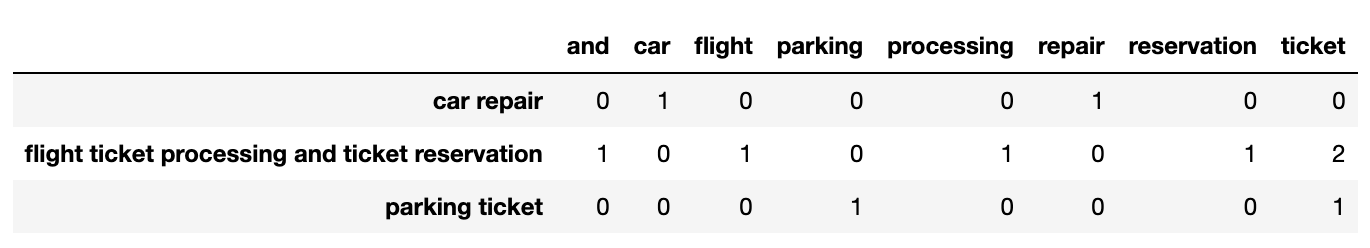
\includegraphics[height=2.9cm]{Bilder/bow.png}

		The result of vectorization are three vectors:
		\[ d_{1} = [0,1,0,0,0,1,0,0] \]
		\[ d_{2} = [1,0,1,0,1,0,1,2] \]	
		\[ d_{3} = [0,0,0,1,0,0,0,1]\]


		This vectorization method can be implemented with ease and in a computationally efficient manner. The \ac{BoW} model allows for a very intuitive understanding of documents, since texts consisting of the same words are considered topically related. 
		
		One of the drawbacks of this method is that no consideration is paid to words being repeated in one document. Additionally, no semantic relationship between words or documents can be inferred. 
		Further, it can be stated, that the \ac{BoW} representation fails to capture the meaning of synonyms. This becomes obvious with an example: document $ d_{1} $ and $ d_{3}$ would be considered to belong into the topic of transportation or automotives. The \ac{BoW} representation suggests topical proximity between document $ d_{2} $ and $ d_{3}$ , through the shared word "ticket". "Ticket" here is used in both the meaning of an entrace pass ($d_{2}$) and in the meaning of a note for a traffic offence  ($d_{3}$). 
		
		To conclude, the \ac{BoW} model is a straightforward text representation method. Still, it fails to capture several aspects of the natural language.
		
		\subsubsection{Tf-Idf}
		The \ac{TF-IDF} model aims to capture more meaning from the corpus by considering the composition of the whole corpus for the calculation of individual document vectors.
		
		\ac{TF-IDF} makes two assumptions about natural language:
		
		\subparagraph{1 Term Frequency}
		
		A word $t_{i} $ which occurs very frequently in one document is considered to describe a text very well. The occurences of one word in one document is denoted as $ \#( t_{i}) $.
		One additional consideration needs to be made regarding the document length. In a document of length $ |d_{2}| = 6 $ and a document of length  $ |d_{3}| = 2 $, the word $ t_{i} $occuring once would be considered equally important to each document. Of course, the word should be considered more important to $ d_{3} $, since it accounts for a larger share of the text. The measure resulting from both ideas is the term frequency:
		
		\[ TF(t_{i}, d_{j}) =   \dfrac{\#( t_{i})}{|d_{j}|} = \dfrac{occurences \; of \; word \; t_{i} \: in \; document \;\:   d_{j}}{legth \; of \; d_{j}} \]
		
		\subparagraph{2 Inverse Document Frequency}
		A word $t_{i} $ which occurs in a large number of documents does not describe one document well. Words occuring in many documents often are articles or pronouns (stopwords) which do not provide value when inspecting the content of a text. The inverse document frequence is a measure accounting for this fact. The inverse document frequency of a word is the proportion between the number of documents in the corpus and the number of documents containing the word. The logarithm is applied, as the importance of a word does not increase proportionally to the number of occurrences.
	
		
		\[ TF(t_{i}, d_{j}) = \log \dfrac{|D|}{\#(d_{t_{i}}) } =  \log \dfrac{number \;  of\;  documents \;  in \; corpus \; D}{ number \; of \; documents \; containing \; word \; t_{i}} \]
		
		Combining both assumptions, the \ac{TF-IDF} measure is created:
		
		\[ TFIDF(t_{i}, d_{j}) \;=\; TF(t_{i}, d_{j}) * TF(t_{i}, d_{j})\]
		
		For the corpus displayed in the previous section the document vectors calculated with the \ac{TF-IDF} measure are:
		
				
		\begin{align}
			&d_1 = & [ 0\;	&0.707107\;	0\;	0\;	0\;	0.707107\;	0\;	0 \\
			&d_2 = & [ 0.39798\;	&0\;	0.39798\;	0\;	0.39798	0\;	0.39798	0.605349 
		\end{align}
			
			\[d_1 = \begin{bmatrix} 0\;	0.707107\;	0\;	0\;	0\;	0.707107\;	0\;	0 \end{bmatrix}	 \\
			d_2 =  \;\begin{bmatrix} 0.39798\;	0\;	0.39798\;	0\;	0.39798	0\;	0.39798	0.605349 \end{bmatrix} \\
			d_3 = \;\begin{bmatrix} 0\;	0\;	0\;	0.795961	0\;	0\;	0\;	0.605349 \end{bmatrix} \]
			
		The \ac{TF-IDF} measure corrects some of the pitfalls of the \ac{BoW} model. It certainly is less vulnerable to skewing by stopwords as words are ranked by importance to each document and the all over corpus. 
		
		Just as the \ac{BoW} representation, \ac{TF-IDF} suffers from high-dimensionality. The vectors contain one element for each word in the vocabulary, resulting in vectors which are inefficient to handle.
		Also, \ac{TF-IDF} fails to represent the topical relationship between $ d_{1} $ and $ d_{3}$. 
		
		\subsubsection{Word Embeddings}
		This lack of "understanding" of related words, and the problem of high-dimensionality is corrected with the third presented option: Word Embeddings.


\section{Modelling}
	\subsection{K-Means with Euclidean Distance}
\section{Evaluation}
	\subsection{Elbow Diagram}
	\subsection{average silhouette method}
	\subsection{gap statistic}
	\subsection{Visualization}
		\subsubsection{PCA}
		\subsubsection{T-SNE}
\section{Deployment}
